%Simple seminar template based on LLNCS document class

\documentclass{llncs}

%general packages
\usepackage[utf8]{inputenc}
\usepackage[english]{babel}
\usepackage[T1]{fontenc}
\usepackage{graphicx}
%generate random text
\usepackage{blindtext}

%set page style
\pagestyle{plain}

% use table package
\usepackage{tabularx}

%math packages
\usepackage{amsmath}

\usepackage{float}

\begin{document}


%define your title
\title{Reinforcement Learning}
\author{Michael Plüss \\ Elias Arnold}
\institute{2016-051-062 (M. Plüss)\\2014-930-770 (E. Arnold)\\
\email{m.pluess@unibas.ch\\elias.arnold@stud.unibas.ch}\\}

\maketitle             


\section{Introduction}
Reinforcement learning attempts to solve the problem of the agent's behaviour in the absence of ground truth data. Such an agent improves its strategy over time and does not need an initial training step. The basic idea is that we feed our agent with a reward based on the agents decisions [Figure \ref{fig:reinforcement_learning}]. Initially, the agent applies actions just with trial-and-error, and then, from these observed rewards, the agent tries to learn an optimal strategy for the environment. In other learning strategies like supervised learning, the agent updates its behaviour based on the ground truth labels from a supervisor. In reinforcement learning, a supervisor is not available anymore. It just replaces these ground truth labels with the rewards from the environment. Remember, that in unsupervised learning neither ground truth data nor rewards were given.\par

Reinforcement learning is a term from psychology and reflects the learning behaviour of nature. For example, animals learn to behave in such a way that hunger is minimized while maximizing hunting success. There are many applications of reinforcement learning in the realm of computer science like image recognition, robotics and computer game AI's.\par

In this summary of chapter 21 from \cite{Russell}, we will first look at the different approaches to designing an agent and then discuss specific methods to implement reinforcement learning. Next we will generalize the insights from the specific methods. Finally, we will take a look at dynamically modifying the strategy, under which the agent operates.

\begin{figure}[H]
	\centering
	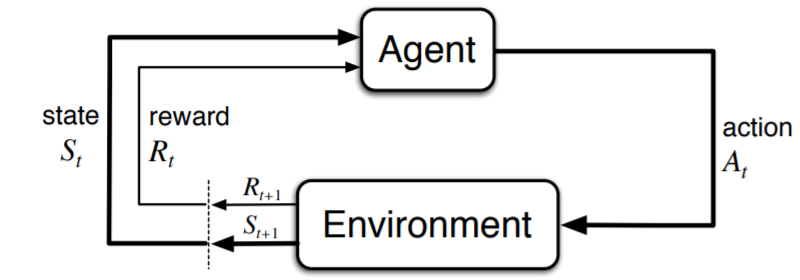
\includegraphics[width=0.6\textwidth]{figures/reinforcement_learning.PNG}
	\caption[caption]{The basic structure of a reinforcement learning agent. The agent finds itself in state $S_t$ and applies action $A_t$. The resulting state $S_{t+1}$ and reward $R_{t+1}$ are fed back to the agent \cite{Sutton}.}
	\label{fig:reinforcement_learning}
\end{figure}

\section{Agent Design}
Depending on the environment we have given, the agent might or might not know the transition model or the reward function of the environment. In reinforcement learning, we assume the case where the agent has no prior knowledge about any of these things. In order to be able to determine suitable transitions, the agent sometimes has to use certain information about the world. The following three agents look at different kinds of information.\par

Throughout this summary, we will refer to such a strategy of the agent as a policy. A policy $\pi(s)\rightarrow a$ is a mapping between a state in the environment $s$ and an applicable action $a$. So it tells the agent which action to execute in a certain state.

% Hmm, when should we introduce the term policy?

%\subsection{Types of Agents}
\subsection{Utility-based Agent}
A utility-based agent takes a state as input and calculates the utility solely from the state. It tries to take the action which moves it to the state with the highest expected utility. Thus, it needs to know which actions are available and to which state these actions will lead. In other words, it needs to learn a model of the environment.

\subsection{Q-learning Agent}
A Q-learning agent learns an action-utility function (or Q-function). This means it learns the expected utility of taking a given action in a given state. Such an agent can compare the usefulness of actions (Q-value) without having to know where these actions take it and thus it does not need to learn a model of the environment. Therefore, we call this agent ``model-free''. A drawback of such an agent is, that it cannot look ahead, because it does not know the successor state where its applied actions lead it to.

\subsection{Reflex Agent}
A reflex agent decides what to do based solely on the current state. It reacts to its environment directly. As such, it does not require a model of the world or the utilities of states or actions. The downside is that such an agent is normally restricted to simple problems. An example would be the AI in a pong game, where it just moves into the direction of the ball. This can be seen as a policy and the agent is therefore ``policy-based''.

% The term "policy" is not introduced yet. Should we delete the last sentence?

\section{Types of Learning}
The goal of the agent is to indicate for each state what the expected reward of a path that leads through the state might be. This is called a utility of a state $U(s)$. The methods to learn these utilities can be divided into passive and active learning.

\subsection{Passive Learning}
In passive learning, the policy is given and fixed. This means that it is predetermined which action the agent should take in each state. In such a situation, we might want to learn the utilities of states or state-action pairs. The goal of passive learning is to label each state with its utility, such that the Bellman equation holds in each state. In contrast to policy evaluation, we assume the action outcome probabilities $P(s'|s,a)$ to be unknown, so we can not just apply the Bellman equation to calculate a states utility.
\begin{align*}
	&U^{\pi}(s)=R(s)+\sum_{s'}P(s'|s,\pi(s))U^{\pi}(s')
\end{align*}
The Bellman equation, where $s$ is the current state, $a$ the applied action, and $s'$ the state in which the agent ends up in. Passive learning just tries to make this equilibrium hold in each state.
%\\ \\
%When considering passive learning, it may sound a lot like supervised learning

\subsection{Active Learning}
In active learning, the agent must additionally find out what to do in each state because the policy is not given anymore. In passive learning, a policy $\pi$ assigns an action $a$ to each state $s$ where the mapping was independent of the states that were already visited. In the active case, the agent must reassess after each transition which action to choose next. The path that the agent has already completed plays an important role in these decisions. One of the main challenges with active learning, is to factor in a certain amount of exploration, where the agent tries to take actions, which were not taken before. The hope is, that by doing so, the agent reaches previously unseen states and possibly discovers a shortcut or a better solution. This topic is discussed in detail in chapter \ref{chap:Balancing}.\par

In active learning, the utilities of the individual states must converge to the Bellman equation too. However, the equation must be adjusted to take into account all executable actions, not just the one which is decided by the policy like in passive learning.
\begin{align*}
	U(s)=R(s)+\gamma\max_{a}\sum_{s'}P(s'|s,a)U(s')
\end{align*}


% TODO: Talk about the bellman equation in the active case

%\section{Passive Learning}
%\subsection{Intro}
%The defining characteristic of passive learning is that the agent has a fixed policy. What this means is that the agent always performs the same action $\pi(s)$ in a state $s$. Remember that this does not mean that the same outcome will always happen, because actions may imply a number of different effects, which occur with different probabilities. The sole purpose of passive learning is then to evaluate the given policy . Specifically, the algorithm learns the utility function $U(s)$ of each state $s$ given the policy . Thus passive learning is similar to policy evaluation, with the difference that a passive learning agent does not know the transition model $P(s'|s,a)$, which describes the probability of reaching state $s'$ from state $s$ with action $a$, nor the reward function $R(s)$, which depicts the reward for state $s$.

%In the next few subchapters, we will look at three different approaches to calculate the utility function.

\section{Algorithms}
So far, we looked at different strategies for the agent to gather the information needed to calculate the current state's utility. We have seen, that these methods can be split up in active and passive learning methods. In this section, we will look at different algorithms to actually calculate the utility values. For each algorithm we will indicate, whether it can be used in active and passive learning.

\subsection{Direct Utility Estimation}
The idea of direct utility estimation (DUE) is to let the agent run several trials and to gradually modify the utility of each visited state after each trial. We use a fixed policy for running the trials and thus, DUE is an algorithm for passive learning. In the longer run, the utility estimate converges to the true values (so that the Bellman equation holds in each state).\par

After each trial, we calculate the utility of each visited state $s$ based on the rewards received by the following states $S_t$  with the following formula:
\begin{align*}
U^{\pi}(s) \leftarrow E[\sum_{t=0}^{\infty}\gamma^{t}R(S_{t})]\text{ where }\gamma\text{ denotes a discount factor and }S_0 = s.
\end{align*}
We do not directly assign the calculated values $U(s)$ to $s$ however. Rather, we keep a running average, that we modify after each trial. This algorithm is very simple, but has a few drawbacks: Firstly, it is not guaranteed to visit every state in the environment (and thus it does not calculate the state's utilities). Secondly, this algorithm ignores dependencies between neighbouring states, which are included in the bellman equation via $P(s'|s,a)$. Consequently, this algorithm converges rather slowly to the true utility values, when compared with other algorithms. However, the absence of these action-outcome probabilities $P(s'|s,a)$ can also be seen as an advantage, because these values are rather hard to estimate from trials.

\subsection{Adaptive Dynamic Programming}
Another algorithm for the passive learning scenario is Adaptive Dynamic Programming (ADP). ADP works similar to direct utility estimation in the way that it also lets the agent run through many trials in order to estimate the utility of the states. The difference to the first approach is, that ADP estimates the transition model $P(s'|s,a)$ from example trials.\par

It achieves this by keeping track of the number of times a state $s$ has been visited and which action $a$ we execute from there in the array $N_{sa}$ and in which state $s'$ we land from there in the array $N_{s'|sa}$. From the ratio of these values we can calculate the probability of reaching state $s'$ from $s$ with the action $a$ as $P(s'|s,a) = \frac{N_{s'|sa}}{N_{sa}}$. This value will approximate the true transition model, given enough trials. Finally, to calculate the utility of each state, we plug our estimated transition model into the Bellman equation for passive learning (with a fixed policy $\pi$):

\begin{align*}
U^{\pi}(s) \leftarrow R(s)+\gamma\sum_{s'}[P(s'|s,\pi(s))U^{\pi}(s')]
\end{align*}

In the formula $\gamma$ again denotes a discount factor.\par

We can modify this algorithm to use ADP in an active learning scenario. In that case, we just plug the estimated transition model in the Bellman equation for the active learning case. The resulting formula looks as follows:

\begin{align*}
U(s) \leftarrow R(s)+\gamma\max_{a}\sum_{s'}[P(s'|s,a)*U(s')]
\end{align*}

Effectively, here we are looking at each possible action $a$ that we can take in a state $s$ and choose the action, which promises the best outcome. This is required, since we do not have a fixed policy anymore. Such a one-step look-ahead approach provides an optimal policy.

\subsection{Temporal Difference Learning}
Temporal-difference learning (TD) is another algorithm to estimate the utility of states in a passive learning scenario.\par

For TD we again use a large number of trials. The idea is, as before in the direct utility estimation, to calculate the utility of a state based on its successor. This time we use the difference of utilities between successive states together with a learning parameter $\alpha$, which becomes smaller as a state is visited more often. The new formula to repeatedly modify the utility values of the states looks like this:
\begin{align*}
U^{\pi}(s) \leftarrow U^{\pi}(s)+\alpha(N_s)*(R(s)+\gamma U^{\pi}(s')-U^{\pi}(s))
\end{align*}
At first glance, this formula looks confusing. If we ignore the learning rate $\alpha$, the equation can be rewritten as $U^{\pi}(s)=R(s)+ U^{\pi}(s')$. Now the closeness to Adaptive Dynamic Programming can be seen.  So in TD we just add $R(s)$ with the utility of the sucessor $U(s')$, while ADP calculates the expected value of the utility of $s'$. $\gamma$ again denotes a discount factor. This algorithm behaves in a similar fashion as the ADP, but requires significantly less computational power.

\subsection{Learning State-Action-Utilities (Q-Learning)}
Another method that is very similar to Temporal Difference Learning, but works in an active learning scenario, is Q-learning. This method learns the utility of state-action pairs ($Q(s,a)$) instead of just the state utilities ($U(s)$), which would not provide any benefits in the passive learning case, since there we have the policy given.\par

The connection between the passive Temporal Difference Learning and the active Q-Learning is given by $U(s)=max_aQ(s,a)$, where $Q(s,a)$ is the utility of action $a$ given state $s$. This allows us to rewrite the Temporal Difference update rule as:
\begin{align*}
	Q(s,a)\leftarrow Q(s,a)+\alpha(R(s)+\gamma*max_{a'}Q(s',a')-Q(s,a))
\end{align*}
$\alpha$ is the learning rate and $\gamma$ is the discount factor.
Note, that when we are in a state $s$ and apply action $a$, we consider all possibly following states $s'$ and actions $a'$ that can be applied next. In other terms, Q-Learning rates a state-action pair only by the best following pair.

\subsection{The SARSA Algorithm}
For the active learning case, there is another alternative to Q-Learning, which also learns Q-values. This method is called SARSA, which is an abbreviation for State-Action-Reward-State-Action $(s, a, r, s', a')$. This algorithm does not consider all pairs $(s',a')$ (like Q-Learning), but waits until an action $a'$ in state $s'$ has actually been executed:
\begin{align*}
	Q(s,a)\leftarrow Q(s,a)+\alpha(R(s)+\gamma Q(s',a')-Q(s,a))
\end{align*}
Because SARSA needs to know in each state $s$ what the following state $s'$ will be, this algorithm is called ``on-policy'', while other Q-learning algorithms which do not need a policy are called ``off-policy''. SARSA converges to the optimal policy, but at a much slower speed than ADP. This algorithm is more realistic than Q-Learning, because it updates a state's Q-value only if $s'$ and action $a'$ are actually visited/executed. (Same difference as between ADP and TD in the passive case)

%\section{Active Learning}

%\subsection{Intro}
%In the Passive-Learning case the agent followed a fixed policy in each trial. Once the agent starts applying actions, the policy $\pi$ was not changed anymore. In the Active-Learning case, the agent considers all possible actions in a state rather than just executing the action recommended by the fixed policy (passive case). For an ADP agent, the update rule becomes:\\
%\begin{align}
%U(s)\leftarrow R(s)+\gamma(\max_{a}\sum_{s'}P(s'|s,a)U(s'))
%\end{align}
%The above formula should remind us of the value iteration algorithm introduced in chapter 17. If we have the optimal U-values, we can also compute the optimal policy with the greedy policy improvement formula (17.4). Can our agent not just follow these optimal actions instead of decide what action to take at each state with the above update rule? Is it enough to just apply the actions suggested by that one-step look-ahead policy?\\
%\\
%To refute this assumption, let us consider an active ADP agent which in every state applies the action recommended by the one-step look-ahead policy improvement formula introduced in chapter 7. In the Active-Learning setting, the agent recalculates the transition model after each action and adjusts the learned policy accordingly (policy improvement). In our running example, it might be that the agent in some trial finds a suboptimal way to the target state (+1) via the states (1,1), (2,1), (3,1), (3,2) and (3,3). The agent improves the expected reward of these states so that this way is more attractive than the optimal way via (1,1), (1,2), (1,3), (2,3) and (3,3). Since this sub-optimal way now seems so promising, it is often passed by the agent. As a result, the utility values of other states that lie not on this way will never be properly learned. Finally, the agent sticks to this suboptimal policy even though the agent starts with the optimal policy! The picture below shows the learned policy (left) and the optimal policy (right).\\
%\\
%\begin{figure}[H]
%	\centering
%	\begin{minipage}{.5\textwidth}
%		\centering
%		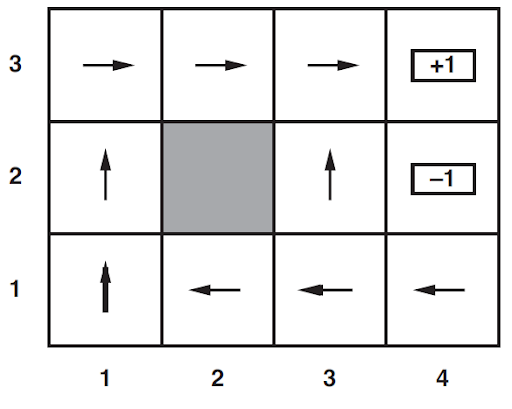
\includegraphics[width=.8\linewidth]{figures/example_policy.png}
%		\label{fig:test1}
%	\end{minipage}%
%	\begin{minipage}{.5\textwidth}
%		\centering
%		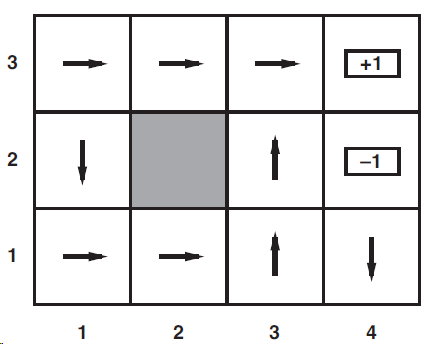
\includegraphics[width=.8\linewidth]{figures/learned_policy.png}
%		\label{fig:test2}
%	\end{minipage}
%\caption{The learned suboptimal policy (left) and the true optimal policy (right). The agent learned a suboptimal policy even though the agent's policy was initialized with the opimal policy.}
%\end{figure}
%The answer to the above question is NO, because of the greedy policy improvement formula:
%\begin{align}
%	\pi^*(s)=argmax_{a \in A(s)}\sum_{s'}P(s'|s,a)U(s')
%\end{align}
%The agent never tries to reach an unknown state which may is a shortcut to a very attractive state. The policy just suggests the best-looking action instead of an unprecedented action that might yet prove worthwhile. Therefore, we have to find a tradeoff between \textbf{exploitation} (maximize the reward) and \textbf{exploration} (apply unseen actions hoping to find a better way). Remember that the goal is to collect as much reward as possible. The exploration of the state-space is overdue, if in the end not a good and worthy trial was found. Therefore, we require an agent to devote himself to optimizing the rewards after a certain period of time. This is known as the \textbf{GLIE} (greedy in the limit of infinite exploration) scheme.\\

\section{Balancing Exploration vs. Exploitation}
\label{chap:Balancing}
With the introduction of active learning, wherein we do not follow a fixed policy but decide where to go before each step of the agent, a new issue emerges: Upon finding a solution, a greedy agent will exploit this solution and steadily fortify the found path. The agent will thus miss the chance to take another route and possibly find a shortcut. The cure to this problem is the introduction of a kind of curiosity via exploration.\par

The basic idea is, that an agent first tries out many different actions, preferring those which it did not take previously. After a while, when the agent has explored the state-space to a reasonable extent, it will shift its behaviour from exploration towards exploitation. Such an approach is called greedy in the limit of infinite exploration (GLIE).\par

As you may suspect, the tricky part is to find the right time when to switch from exploring to exploiting.\par

One way to implement such a GLIE scheme is to introduce a probability to take a random action instead of the greedy one. This function must decay over time to fit the GLIE constraints, for example $\frac{1}{t}$.\par

Alternatively, you can assign a reward function $f$ to a state instead of a constant reward. This function gives a state a reward (makes the state more attractive) depending on the number of times this state was already visited. A possible implementation would be:
\begin{equation*}
	f(u,n)=\begin{cases}
	R^+ \text{ if } n<N_e\\
	u \text{ otherwise }
	\end{cases}
\end{equation*}
 

%\begin{align}
%	f(u,n)=\begin{cases}
%		R^+&if n<N_e\\
%		u&otherwise
%	\end{cases}
%\end{align}

Where $R^+$ is an optimistic estimate of the best possible reward that any state can have, $n$ indicates how often a state has been visited, $N_e$ is some constant threshold, and $u$ is the “classical” utility of a state according to the Bellman equation.\par

% With this, we can rewrite the ADP update rule to:

%\noindent Where $R^+$ is an optimimistic estimate of the reward of a state, which has been visited less than $N_e$ times. The ADP update rule then becomes:
%\begin{align}
%U^+(s)\leftarrow R(s)+\gamma max_a f(\sum_{s'}P(s'|s,a)U^+(s'),N(s,a))
%\end{align}
This formula makes unvisited states artificially appear attractive to the pathfinding algorithm (with $R^+$). But if after $N_e$ attempts via this (initially unexplored) state no better trial is found, the state is assigned with his original reward.\par

A possible application of this function is for example to modify the update rule of the ADP algorithm, which then becomes:

\begin{align*}
U^{+}(s) \leftarrow R(s)+\gamma\max_{a}f(\sum_{s'}[P(s'|s,a)*U^{+}(s')], N(s,a))
\end{align*}

By using $U^{+}$ we signify, that we use a version of the ADP algorithm, wherein we use the modified rewards of states.

%\subsection{Learning state-action-utilities (Q-Learning)}
%Remember that in the Passive Learning case, the main idea behind Temporal Difference Learning was that we do not need a model. The fixed policy in each state made it clear which action would be executed next. Since we are now in the Active Learning case where we do not have a fixed policy and have to make a decision in each state, this is no longer possible.\\
%\\
%However, there is another method that is very similar to Temporal Difference Learning, but works without an underlying model. This method learns the utility of state action pairs instead of just the state utilities. The method we are talking about is called Q-Learning. The connection between the (passive) Temporal Difference Learning and the (active) Q-Learning is given by $U(s)=max_aQ(s,a)$, where $Q(s,a)$ is the utility of action $a$ given state $s$. This allows us to rewrite the Temporal Difference update rule as:
%\begin{align}
%	Q(s,a)\leftarrow Q(s,a)+\alpha(R(s)+\gamma max_{a'}Q(s',a')-Q(s,a))
%\end{align}
%Note, that when we are in a state $s$ and apply action $a$, we consider all possible states $s'$ and actions $a'$ that can be applied next. In other terms, Q-Learning rates a state-action pair with the best following pair only. 

%\subsection{The SARSA algorithm}
%Nonetheless, there is a more realistic algorithm than Q-Learning, which also learns Q-values. This is called SARSA, which is an abbreviation for State-Action-Reward-State-Action ($s, a, r, s', a'$). This algorithm does not consider all pairs $(s',a')$ (like Q-Learning), but waits until an action $a'$ in state $s'$ has actually been executed:
%\begin{align}
%	Q(s,a)\leftarrow Q(s,a)+\alpha(R(s)+\gamma Q(s',a')-Q(s,a))
%\end{align}
%Because SARSA needs to know in each state $s$ what the following state $s'$ is, this algorithm is called "\textbf{on-policy}", while other Q-learning algorithms which do not need a policy are called \textbf{off-policy}. SARSA converges to the optimal policy, but at much slower speed than ADP. This algorithm is more realistic than Q-Learning, because it updates a states Q-value only if $s'$ and action $a'$ are actually visited/executed.
% However, the tradeoff is that SARSA needs an initial policy (we do not iterate over all possible $Q(s',a')$) which then gets updated (eg. with the greedy policy improvement formula (17.4)). SARSA is called “\textbf{on-policy}”, while Q-Learning is called “\textbf{off-policy}”. In our running example, the 4*3 grid world, both SARSA and Q-Learning converge to the optimal policy, but at much slower speed than ADP. Imagine that we may not have full control of our agent. In such a situation is is better to learn a Q-value according to the actions that is actually executed (SARSA), than a Q-value according to the action which would be the best (Q-Learning). Therefore, SARSA is more realistic, while Q-Learning is more flexible.

\section{Generalization in Reinforcement Learning}

%\subsection{Intro}
In the previous chapters we discussed methods to calculate state(-action)-utilities for every state the agent can end up in. We had to consider all possible successor states/actions to come up with the true utility estimate for a state. While ADP converged to the optimal policy relatively quickly, Temporal Difference Learning, and SARSA take much longer. Since we do not have a model in these cases, we have to consider a lot sample trials for the optimal utility estimate.\par

%For our running example - the 4*3 grid world - these were reasonable approaches.
These approaches are reasonable for small state-spaces.
On the contrary, if the state-space were large, it would no longer be justifiable to calculate the utility estimate for each state in this way. Therefore, it is often attempted to approximate the true utility of a state with a function that can be evaluated in one sweep. Such a function approximation has the following form:
\begin{align*}\label{eq:generalisation}
	\hat{U}_{\theta}(s)\leftarrow \theta_1f_1(s)+\theta_2f_2(s)+...+\theta_nf_n(s)
\end{align*}
The $f$’s are called features and the $\theta$’s are called the parameters of the evaluation function $\hat{U}_{\theta}(s)$. The main benefit of function approximation is the ability to generalize from a few states where the true utility estimate is known to a larger state-space where we cannot calculate the utility of every single state. For example, the state-space of the game backgammon contains $10^{20}$ states. Tesauro~\cite{Tesauro} showed in 1992 that a computer program could play backgammon as well as a human, with a function approximation that could only model $10^{12}$ different states. The $f$’s are fixed functions of the state variables, that are weighted by their respective $\theta$s. These $\theta$s need to be adjusted after each trial (idea of reinforcement learning). For example, we can use the
Widrow-Hoff rule (also called ``Delta rule'') to update the parameter $\theta_i$:
\begin{align*}
	\theta_i \leftarrow \theta_i-\alpha\frac{\partial E_j(s)}{\partial\theta_i} \text{ where }E_j(s)=\frac{(\hat{U}_{\theta}(s)-u_j(s))^2}{2}\text{ (MSE) } 
\end{align*}
In the above equation, $u_j(s)$ denotes the observed utility of a state $s$ in the j-th trial and $\hat{U}_{\theta}(s)$ denotes the predicted utility, according to formula \ref{eq:generalisation}. The $f$’s are usually functions of the form $f_i(x,y)$, where $x,y$ are features of the state, that are weighted by $\theta_i$. A common choice is a function that returns the agents closeness to the state with the highest reward. Let us consider a grid world of the size $100^2$ and the state with reward “+1” has the coordinates (50,50). Then, $\hat{U}_{\theta}(s)$ may look like:
\begin{align*}
	\hat{U}_{\theta}(s)=\theta_1f_1(x,y)=\theta_1\sqrt{(x-50)^2+(y-50)^2}
\end{align*}
Here, the utility of a state depends solely on the distance to the goal state, weighted with $\theta_1$.

\section{Policy Search}
%\subsection{Intro}
The general idea of policy search is to change the policy for as long as there is improvement and then stop. Normally, we want to work with policies $\pi$ that are parametrized. We apply the changes to the parameters $\theta$. Usually, such policies have a lot fewer parameters than there are states in the state-space of the problem. This ensures a certain degree of generalization and also makes it much easier to mathematically work with the policies. As an example, we could define the obvious policy which always takes the action $a$ from the state $s$ that predicts the biggest reward. This would result in a greedy agent, that never explores unseen states.

\subsection{Problems}
A problem that we have to be aware about when using policy search, is that the policy may be a discontinuous function. The problem with that is that small changes in $\theta$ may lead to very different outcomes. To illustrate this, let us picture an example where a small change of $\theta$ leads an agent to take the left path, instead of the right one. Because the agent took another path at the intersection, it now lands in another goal state with a considerably higher reward. This “jumpy” behaviour of the policy function can make it very difficult or even impossible to take its derivative, which we need to perform optimization techniques such as hill-climbing. Luckily, we can tackle this problem by using a stochastic policy representation $\pi_{\theta}(s,a)$, which gives us a probability of selecting action $a$ in state $s$. An often-used approach to achieve this is the softmax function:
\begin{align*}
	\pi_{\theta}(s,a)=e^{Q_{\theta}(s,a)}/\sum_{a'}e^{Q_{\theta}(s,a')}
\end{align*}

\subsection{Policy Improvement}
How do we now actually improve the policy? To evaluate how good our policy actually is, we need a function $\rho(\theta)$, called the policy value, which represents the expected reward for executing the policy $\pi_{\theta}$. If we are able to find an expression for $\rho(\theta)$ in closed form, this becomes a standard optimization problem and we can simply follow the policy gradient $\nabla_{\theta}\rho(\theta)$, provided $\rho(\theta)$ is differentiable, but oftentimes this is not possible.\par

An alternative is to execute the policy $\pi_{\theta}$ and take the accumulated reward of the trial as the value for $\rho(\theta)$. In this situation, we can observe the change of $\rho(\theta)$ for small changes of $\theta$ and apply the change which results in the biggest improvement of $\rho(\theta)$.\par

When we have a situation where the environment or the policy is stochastic, this becomes a bit more complicated. Executing two trials with the same policy may lead to very different outcomes, because the path that the agent takes is not deterministic anymore. The solution is to run several trials and take the average of the accumulated rewards as $\rho(\theta)$. The drawback of this approach is, that it may be very expensive, time-consuming or even dangerous to run a trial, so this is not always an option.
Luckily it is possible to obtain an unbiased estimate of the gradient $\nabla_{\theta}\rho(\theta)$ at $\theta$. We will assume a nonsequential environment in which the reward $R(a)$ is collected directly after taking action $a$ in the start state $s_0$. Here, $R(a)$ stands for the sum of subsequent rewards in the trial(s) where we chose action $a$. This algorithm is called ``REINFORCE'' (Williams, 1992)\cite{Williams1992} and is usually much more efficient than standard hill-climbing.
%In this situation, the policy value equals the expected value of the reward, leading to the following formula:
%\begin{align}
%	\nabla_{\theta}\rho(\theta)=\nabla_{\theta}\sum_{a}\pi_{\theta}(s_0,a)*R(a)=\sum_{a}(\nabla_{\theta}\pi_{\theta}(s_0,a))*R(a)
%\end{align}
%For this formula, there exists a trick to approximate the policy gradient. For this, we define $N$ as the number of trials that we take and $a_j$ as the action that we take in the j-th trial. This leads to the following simplification:
%\begin{align}
%	\nabla_{\theta}\rho(\theta)=\frac{1}{N}\sum_{j=1}^{N}\frac{\nabla_{\theta}\pi_{\theta}(s,a_j))*R_j(a)}{\pi_{\theta}(s,a_j)}
%\end{align}
%for each state $s$ visited, where $a_j$ is the action taken on the j-th trial and $R_j(s)$ is the total reward received from state $s$ onwards in the j-th trial. This algorithm is called \textbf{REINFORCE} (Williams, 1992) and is usually much more efficient than standard hill-climbing.

%\subsection{Correlated Sampling}
%There is another way to compare two policies. Consider the situation where we have two different policies for playing blackjack and we wanted to know which one was better. If we just let them play $N$ games against a standard “dealer”, we might get unreliable results of their performance because the result of the game is greatly determined by the hand that they’re dealt. The solution is quite simple: Precompute $N$ hands of cards and let both policies play with the same cards. Only when they use the same cards, the resulting performance is comparable. This method is called correlated sampling and works as the basis of the \textbf{PEGASUS} (Ng and Jordan, 2000)\cite{Ng00pegasus:a} algorithm.
%This algorithm can be used for domains where a simulator is available such that the “random” outcomes of actions can be repeated. The algorithm works by precomputing $N$ sequences of random numbers. The policies that we want to compare all use these same sequences as the basis of their trials. Interestingly, the number of sequences that we need to ensure that the value of every policy is well estimated only depends on the complexity of the policy space and not on the complexity of the domain.

\subsection{Conclusion}

In this chapter, we have learnt how to use reinforcements (rewards) to learn utilities or policies. For that we have looked at different ways to design agents (focusing on the utilites of states vs. state-action pairs) and different algorithms to compute the utilites. These algorithms can be used in different settings: In a passive setting where the policy is given and fixed, or in an active scenario, where the policy is not given and has to be found.\par
Furthermore we have looked at the issue of exploration vs. exploitation, where the difficulty lies in balancing the curious exploration of unknown states vs. greedily moving towards the most attractive state.\par
We also discussed the generalization of utility and/or policy calculation, such that we can use reinforcement learning with big state-spaces, where the  previously discussed mehtods would not be feasible. Learning parameters of base functions also enables the abstraction of a state's utility based on its features. This has the advantage, that we can already estimate the utilities of states that we see for the first time.
\\\par
In practice, reinforcement learning has proven to be a viable learing strategy. Reinforcement learning has applications in robotics, games and chemistry, making it a very flexible concept with veritable benefits.
\\\par
``There is no reasoning, no process of inference or comparison; there is no thinking about things, no putting two and two together; there are no ideas - the animal does not think of the box or of the food or of the act he is to perform.''\\
- Edward Thorndike \cite{thorndike1965animal}, the psychologist who proposed Law of effect.
%Citation from: https://towardsdatascience.com/applications-of-reinforcement-learning-in-real-world-1a94955bcd12


\newpage

%bibliography
\bibliographystyle{splncs03}
\bibliography{bibliography}

\end{document}